
\documentclass[12pt,a4paper]{article}
\usepackage{indentfirst}
\usepackage{CJK}
\usepackage{color}
\usepackage{graphicx}


\begin{document}
\begin{CJK}{UTF8}{gbsn}
\CJKindent

\begin{titlepage}
\begin{center}
\textsc{\Huge 云计算应用开发课程}\\[0.5cm]
\textsc{\LARGE 应用项目计划书}\\[2.5cm]

\begin{tabular}{ |l|l| }
	\hline
	项目名称: & 基于云计算的自助旅游详细方案订制\\ \hline
	队长姓名: & 龚睿奇\\ \hline
	队长电话: & 13631239412 {\slash} 659412\\
	\hline
\end{tabular}
\end{center}
\vspace{10cm}
\begin{center}
\begin{tabular}{ |c|c|c| }
	\hline
		 & 姓名   & 学号	\\ \cline{2-3}
	团队成员 & 龚睿奇 & 12353048	\\ \cline{2-3}
		 & 乔丹   & 12353???	\\ \cline{2-3}
		 & 杨奇标 & 12353???	\\
	\hline
\end{tabular}
\end{center}

\end{titlepage}

\section{应用介绍}
	% section 1.1
	\subsection{背景介绍}
	如今,人们的精神生活日趋丰富,逢年过节外出旅游是常有的事情。对于学生群体及上班一族而言,趁着周末在城市的周边或郊外进行短途旅行,亦很常见。随着人们对旅行的要求不断提高,由传统旅行社提供的传统意义上的“跟团“旅游服务,其缺点和不足日趋显现,已经不能满足一部分人的需求。因此,”自助游”这种旅游方式,即由自己来定制旅行的全过程,包括要去的景点,日程的安排,交通方式的选择,食宿的安排等应运而生。“自助游”的这种个性化,全定制的旅行方式十分地诱人,因此也赢得了广泛的欢迎。但是其缺点也很突出,概括而言就是一个词---“麻烦”:一切的饮食、住宿、交通等细节,都需要由自己来安排。这对一些没有接触过“自助游”的人来说,还是相当有门槛的。人们不仅仅要消耗额外的时间和精力去规划行程,而且在规划行程的过程中,很可能使用了错误或过时的信息,造成规划失误,以至于最终旅途不顺,甚至造成财产损失。正是“自助游”的这些缺点所带来的风险和不确定性,导致还有相当一部分人对其心存芥蒂。

	经过讨论和分析,我们发现,人们在策划旅行的时候,真正需要去关心的,仅仅是那些要参观的景点,以及那些要进行的旅行体验;而至于除此以外的其他方面,例如交通,饮食及住宿等细节\footnotemark,都不属于旅行真正有意义的部分。而当一个用户选择了“自助游”,并且在规划自己的旅游行程时,他关心得更多的,却是这些不重要的“细枝末节”;并且,上述的“自助游”的风险和不确定性,也大多出自于此。鉴于此,我们认为,这其中存在着不合理性。而我们的这个应用,正是要去解决这不合理之处。

	\footnotetext{需要说明的是,很多时候,“食、住、行”三者本身也是旅行的意义所在。但这部分,我们将其归纳到前述的“旅行体验”中,此处所指的是除这些以外的部分。}

	% section 1.2
	\subsection{功能介绍}
	我们这个应用的目的,就是为用户订制完备及详细的“自助游”旅行方案,省去用户处理旅途细节的忧虑及烦恼。用户在使用这款应用,来规划自己的“自助游”方案时,只需要提交以下信息:
	\begin{itemize}
	\item 希望前往的地点(城市);
	\item 有兴趣的景点或体验项目;
	\item 旅途时间,预算等少量其它信息,
	\end{itemize}
	我们的应用程序就可以根据用户提交的要求,为用户制定一份完整且详细的“自助游”方案。该方案具体将包括以下内容:
	\begin{itemize}
	\item 旅行日程(哪一天参观哪些景点);
	\item 食宿安排(用餐地点,酒店的位置);
	\item 交通规划(交通方式及各段交通耗时);
	\item 注意事项等其他信息,
	\end{itemize}
	并且将以顺序表或流程图的形式,直观地向用户展示我们的推荐方案。当然,用户拥有最终决定权,在我们呈现了推荐方案后,用户可以继续根据自己的需要来修改这份方案,直到自己满意,并做出最终的决定。方案被制定好以后,相关文件会在云端及用户本地分别保存,不仅增加了设备无关性,也防止在旅行途中由于上不了网而无法随时查看。
	
	% section 1.3
	\subsection{现有应用}
	必须承认,如今市面上已经有不少旅游相关的软件、手机应用及网站。我们收集了一些关于它们的统计数据,以便于了解现有应用的总体情况。这些体现数据的图表,我们将它们呈现如下:

	\begin{center}
	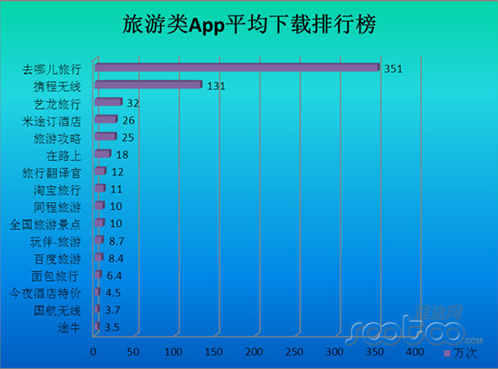
\includegraphics[scale=0.8]{image1}
	\end{center}

	旅游类App平均下载排行榜,该图引自《2012旅游类app应用市场分析报告》。

	从上图中我们可以看到,旅游类App应用程序呈现多样化的发展趋势。就类别而言,上图呈现的应用有如下几种:
	\begin{itemize}
	\item 综合性的旅游App,如去哪儿旅行、淘宝旅行等;
	\item 专门提供预定服务的预订类App,如米途订酒店、国航无线等;
	\item 旅游攻略类App,如旅游攻略;
	\item 语言翻译类App,如旅行翻译官;
	\item 旅游分享类App,如在路上等。
	\end{itemize}

	劲旅网发布2014年6月国内预订类旅游App下载量TOP10
	\begin{center}
	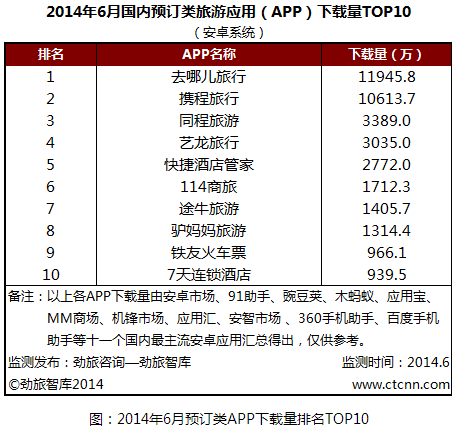
\includegraphics[scale=0.8]{image2}
	\end{center}

	劲旅网发布2014年6月国内分享类旅游App下载量TOP10
	\begin{center}
	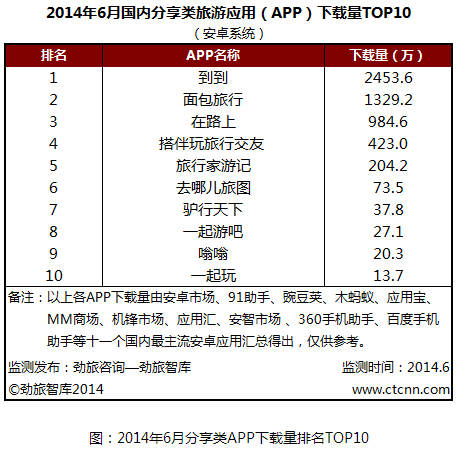
\includegraphics[scale=0.8]{image3}
	\end{center}

	劲旅网发布2014年6月国内工具类旅游App下载量TOP10
	\begin{center}
	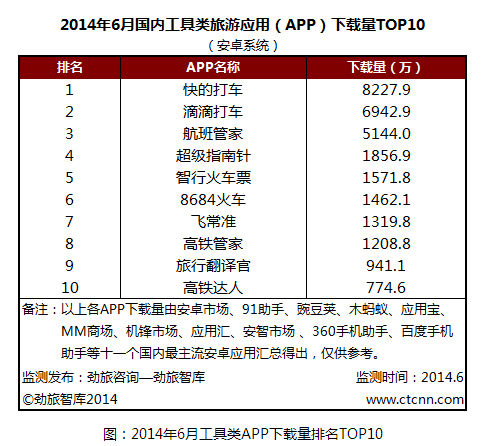
\includegraphics[scale=0.8]{image4}
	\end{center}

	劲旅网发布2014年6月国内攻略类旅游App下载量TOP10
	\begin{center}
	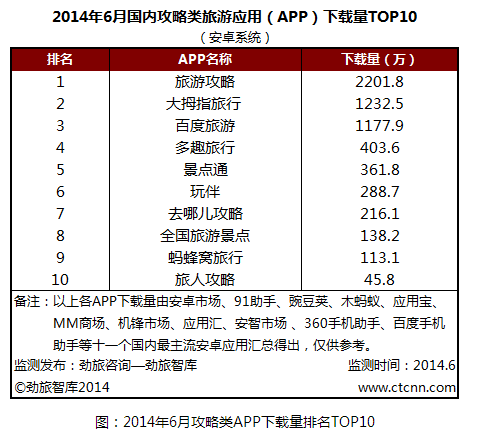
\includegraphics[scale=0.8]{image5}
	\end{center}

	从下载量可以看出,预定类的旅游应用已经占据了很大的市场份额,而且已经发展相当成熟了。所以我们的应用就不再涉及这一方面。	

	对比而言,分享类旅游应用的下载量在这几类中相对较少,说明其市场需求并不高,并且无法和大的分享通讯类应用相比,如微博、微信、QQ空间等,所以我们的应用也就不囊括这项多余的功能。	

	而工具类旅游应用的下载量也是几类别中较高的,说明其具有一定的实用性及市场需求量,在这一方面我们的应用会涉及到公交路线的规划,以及天气等其他旅游注意事项的提醒。

	最后,我们发现攻略类旅游应用的下载量最少,通过调查并非攻略类应用毫无需求,而是这类应用通常华而不实,仅仅是提供超量而杂乱的旅游信息,众多用户评价烧流量,信息更新速度慢,占用较大的手机运行内存。所以在这一方面,我们的应用将会做出较大的创新和改进,相信会吸引来更多这这方面需求的用户。

	对于现有应用的优缺点分析:
	\begin{itemize}
	\item 以导航路线为主的应用有:谷歌地图、百度地图、爱帮公交等。这些应用需要即时查找和定位,虽然信息丰富完整,但是用户需要花费大量的时间和流量;在旅游途中使用时,用户需要在路上一边行走,一边拿着手机查询,因而错过了美丽的风景;
	\item 以酒店、车票预定为主的应用有:携程旅游,去哪儿网等。这些应用虽然囊括功能全面,信息丰富,便于交易,但是也存在一定的安全问题,信誉问题,同样也会使手机应用显得过于冗杂;
	\item 以旅游攻略为主的应用有:旅游攻略、携程旅游等,虽然是旅游攻略,但是也仅仅是限于景点的推荐介绍,局限于为用户呈现相关的信息;
	\end{itemize}

	% section 1.4
	\subsection{创新之处}
	上面列举了不少旅游相关的网站及应用。总体而言,现有的旅游相关应用在种类上而言已经算是应有尽有了,但是它们更多的是停留在信息查询,交易支付,交流互动等需要实时操作,并且花费大量流量和时间的功能服务上面,这样反而影响的旅行的真实体验。	

	我们并没有发现一款软件或者应用,可以像旅行管家一样,在旅行开始前就可以根据用户的需求制定一份较为详尽,并且足够优化的旅行行程安排,其中包括旅行日程、食宿安排、交通规划、注意事项等其他信息。用户只需在旅途中随时打开这个简洁的行程表即可,不需进行过多的查询搜索操作,也不用浏览到很多不必要的信息,也就是说做到了完全的离线使用,节省了大量的流量,以及宝贵的旅行时间。有了一份事先规划好的旅行计划,用户就可以更好地享受到完整而丰富的旅行体验了。	

	总而言之,我们的应用有以下几点亮点:
	\begin{itemize}
	\item 自动规划最优行程,用户不需过多思考,节省宝贵的旅行时间;
	\item 离线查看详细行程,节省浏览查询的流量消耗;
	\item 按需所呈,而非一次呈现所有的旅游信息;
	\item 应用简洁不冗余,节省众多广告等必要的流量消耗,以及手机负载;
	\end{itemize}	

\clearpage
\section{开发方案}

	% section 2.1
	\subsection{实现方案}
	在阐述我们的实现方案之前,有必要简要说明一下我们预想的这个应用的使用流程。在阐述完使用流程后,我们将结合使用流程,来讲解这个应用的具体实现方案。

	首先,这个应用大体的使用流程列举如下:
	\begin{enumerate}
		\item
		用户选定旅游目的地,具体到城市名,并且提供旅游预算,旅行时间等信息;
		\item
		应用展示该城市内及周边的景点,以及景点相关的信息,供用户挑选;
		\item
		根据用户的选择,为用户规划路线,安排行程及食宿,向用户呈现一份推荐方案;
		\item
		用户对方案进行修改后,保存。
	\end{enumerate}
	
	其次,按照我们的设想,我们的应用将会由两个部分组成:用户手机中的应用软件(客户端),以及架设在云端的服务器。其中,正如大多数的云应用一样,本地的客户端,即用户手机中的应用并不进行太多的运算和操作,仅仅是为用户提供一个图形界面,收集用户的输入信息,并将这些信息上传到云端,由云端进行处理。云端处理完毕得出结果以后,将其发回给本地的客户端。本地的客户端对传回的数据进行一定的图形渲染,并最终以图形化的形式呈现给用户。因此,结合上述的使用流程,具体的应用整体实现方式如下:
	\begin{description}
	\item[建立云端数据库] \hfill \\
	这是搭建本应用的第一个步骤。我们认识到,如今已经有不少旅游相关的网站和信息提供者。因此,我们不需要生成我们自己的数据,只需要将已有应用的数据收集并整合起来,例如借助百度地图的API搜集地理信息,从大众点评网收集对餐厅和酒店的评价,从旅游地的当地政府部门网站中收集景点及政策的相关信息等。云端的一些优点,例如24小时不关机,网络带宽大,廉价且弹性存储空间等,就可以在这里被运用:我们可以将“爬虫”程序部署在云端,以比较优良的网络带宽,连续不断地收集并更新云端的数据,然后将这些数据,放到云端的数据库管理系统(DBMS)中进行维护和管理。对于“爬虫”程序,网络上已经有不少现有的程序可供修改和使用,我们设想的是使用Python语言来实现,而DBMS则使用MySQL。
	\item[前期交互] \hfill \\
	在手机App中保存一份中国城市的列表,用户在UI界面中选定其中一个城市,并设置一些附加信息。用户输入完毕后,App将用户输入的信息上传到云端,云端根据一些内置数据及由其他地图应用获取的数据,收集选定城市周边的景点,将这些景点信息回传给用户。用户在手机App中选择好感兴趣的景点后,App向云端发送少量数据,指定这些景点。
	\item[决定景点的优先级] \hfill \\
	由于各个景点之间存在差异,为每个景点都分配同样多的时间,显然不是个好主意。因此云端先根据一套事先做好的,内置的标准,对这些景点做出区分并排序,排名靠前的景点,需要被安排比较多的时间,并且对它的行程要被安排得比较早。当然,在这个排序的过程中,用户对各个景点的偏好也应该被考虑。我们可以让用户在选择景点的时候顺便附上感兴趣的程度。
	\item[景点日程安排] \hfill \\
	包括各个景点的游览时间,以及前后景点之间的交通线路规划。在旅行的过程中,游客自然不希望在路途上花费大量的时间。这意味着,在安排日程的时候,我们需要对用户指定的景点按照它们的地理位置进行聚类,相互邻近的景点可以被连续地安排在一起,这样就可以减少用户耗费在路途上的时间。
	\item[食宿安排] \hfill \\
	安排好了景点的日程之后,就可以根据若干景点的地理位置,搜索其附近的餐饮及住宿服务。在搜索餐厅和旅馆的时候,也不需要对所有景点的周边都进行搜索,而只需要在那些安排于用餐时间前后游览的景点周边进行搜索。这么做,不仅减少了搜索量,降低了运算量,而且还有利于用户获得更人性化的旅游方案。这一步以及前两个步骤,我们计算使用C{\slash}C++程序,结合MySQL对C语言的API接口来实现。
	\item[整理并回传方案] \hfill \\
	至此,一份推荐给用户的方案就基本上在云端制作完成了。这份方案预计会以文本文件的形式被生成出来,云端需要将这份推荐方案回传到用户的手机App上,而手机上的App则读取这份文本文件,通过编排和渲染,以用户友好的方式将我们推荐的方案完整地呈现出来。数据回传的过程,我们预计使用云计算实验课上介绍的Python语言的webpy库,或者也可以用C语言程序创建一个Socket来实现。
	\item[用户修改并确认] \hfill \\
	用户可以细致地浏览这份方案,并且修改其中的任何细节。在用户修改完毕点击确认之后,如果原先的方案有被修改过,那么修改过后的方案文件会被上传到云端,同时也会在用户的手机中保留一份副本,方便用户快速地查看和浏览。
	\end{description}

	最后就是云平台的选择。综上所述,我们应用的实现,在云端要运用到Python,MySQL以及C{\slash}C++程序,并且还有一个用Java+XML实现的Android应用程序。可见,我们的云端必须是一台支持多种语言,而且功能相对完备的虚拟机。在选择云服务提供商的时候,我们必须选择那些可以在云上架设虚拟机的服务商。在云计算实验课上,TA们向我们展示了一些公司提供的云服务,其中最符合我们需求的,无疑是微软的Windows Azure。它提供的是一台配置可供选择的云端虚拟机,我们可以在上面做一切能够在本地PC上做的事情,例如运行操作系统,安装软件,配置开发环境等等。在Windows Azure上不仅可以选择虚拟机器的配置,还可以选择要安装的操作系统。根据我们的需求,我们认为Ubuntu 14.04LTS操作系统是我们的首选,因为它对上述三种语言都有很好的开发以及运行环境支持,并且对网络和内存的管理都比较好。
	
	% section 2.2
	\subsection{可行性分析}
	\begin{description}
	\item[市场可行性] \hfill \\
	我们的App,主要是针对非随团旅游的旅游者,为他们提供一整套可供选择的旅游必需信息,包括旅游景点推荐、天气适宜条件、旅游路线选择、住宿选择定位导航、饮食场所定位导航等。每一个不喜欢随团旅游,又不想花费太多时间自己做旅行计划的人都是我们的潜在顾客,并且,这是一个庞大的、需求仍未被满足的消费群体。
	\item[产品可行性] \hfill \\
	a. 产品设计

	我们的App是建立在当前众多网络查询服务的基础之上的。这些提供数据的网站包括旅游网、百度地图、美团网、天气网等,因而我们可以获取到足够多的数据。 
	\clearpage
	百度地图:
	\begin{center}
	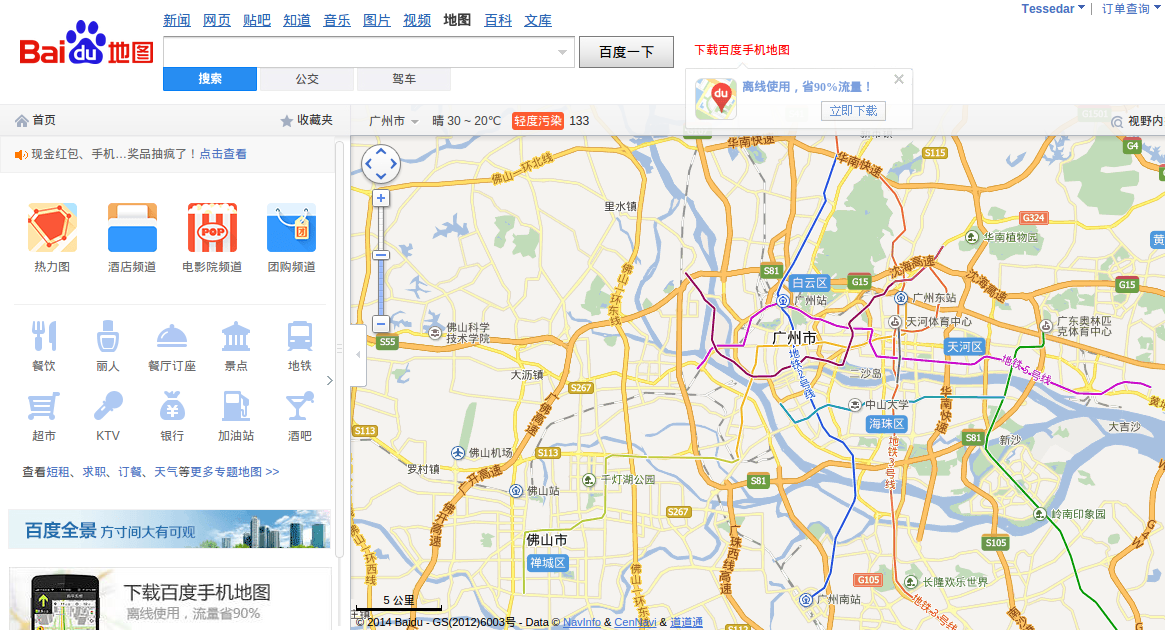
\includegraphics[scale=0.3]{BaiduMap}
	\end{center}

	美团网:
	\begin{center}
	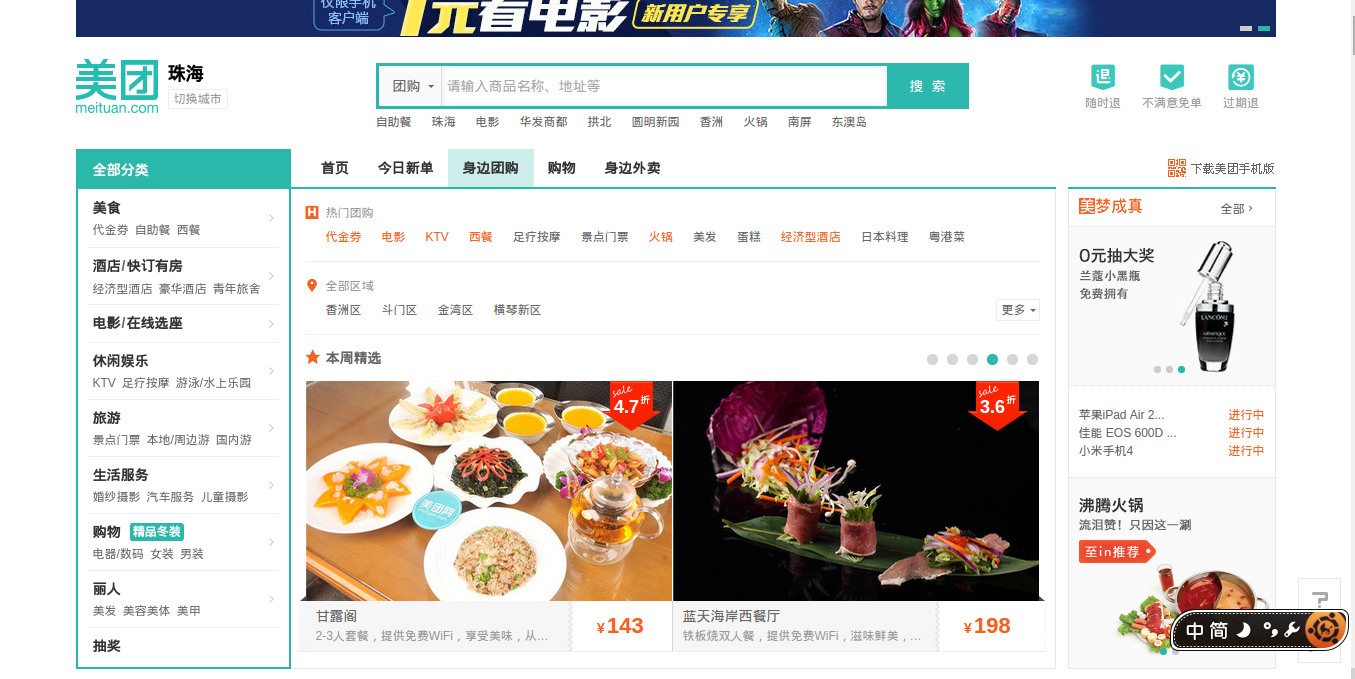
\includegraphics[scale=0.3]{Meituan}
	\end{center}

	b. 产品优势

	我们的App的优势在于提供的是一整套的服务信息。 当前市场上,所有的产品都只是提供一个或两个方面的服务,他们的服务,不可谓不精心。譬如,百度地图所能提供的,定位附近所有的餐厅、旅社等。但是,我们有足够的理由相信,用户出去旅行还想要时不时上网查询。这不仅会浪费用旅行的时间,而且还会影响兴致,特别是突然面临查不到想要的结果的困境时。而我们的App,虽然不能像这些市场已有的产品那样,把单个服务做精、做全面。但却提供了一整套可行的方案可供选择。用户只需要在未出行时使用我们的App进行查询和选择,就能最终得到一张图表,是其旅行计划的一整套信息所在。因而,再不需要去到一个地方再询问有哪些景点,也再不用旅游途中还为去哪儿吃去哪个住而犯愁,更不用面临忽然断网而查不到相关信息的窘境。
	\item[技术可行性] \hfill \\
	按照我们的设想,这个应用中需要用到的一些技术,以及需要解决的问题,都会被严格地控制在我们当前的能力范围之内;如有超出的部分,则会适当地进行简化。此部分的详情,请参见2.3节“关键技术问题”及2.4节“开发进度安排”。
	\item[性能可行性] \hfill \\
	我们的App的主要服务是运行在云端主机上的,用户只需要下载较小的一个App前端,就可以在出行前通过简单的点一点获取大量的旅游指南信息。方便快捷,简单高效。
	\end{description}

	% section 2.3
	\subsection{关键技术问题}
	我们这个应用开发起来,还是有一定难度的,需要解决不少技术上的问题。下面将对已经考虑到的技术问题进行阐述。
	
	\begin{description}
	\item[收集网络上已有的信息,整理组成云端数据库] \hfill \\
	云端是一台24小时运行的虚拟机,它可以不间断地运行,收集大量的信息。云端需要收集的信息,大概分为以下几个类别:
		\begin{enumerate}
		\item	旅游网站提供的景点信息;
		\item	地图网站提供的地理坐标及周边环境信息;
		\item	点评类网站提供的客户评价信息;
		\item	景点官方网站或地方政府网站的法律及旅游政策信息。
		\end{enumerate}
	
	要收集网络数据,则离不开所谓“爬虫”程序。我们预计在网络上应该会有不少现成的“爬虫程序”的Python源代码,只要下载下来并做一定的修改,应该就可以使用了。因此,“爬虫”程序的问题不难解决。

	不难想象,所谓的“爬虫”程序,就是以一个信息量大的网页(例如门户网站首页)为起点,以各个网页中存在的url链接为对象,使用搜索算法逐个访问每个页面,并获取上面的信息。可以想象,被“爬虫”程序收集下来的数据是原始的html文本,还夹杂着用网页脚本语言实现的例如动态广告及图片等冗余信息。我们必须通过一些软件及算法,对收集回来的原始数据进行处理,将其中那些冗余的数据去除掉,提取出关键的、有用的信息。由于我们小组的成员没有做过数据挖掘方面的工作,因此提取有效信息这部分的工作,对我们来说是很具挑战的。
	
	\item[对景点优劣进行排序的方案和标准] \hfill \\
	这部分,是整个整个应用最最关键的步骤,其地位可以说是“承上启下”:承接上述收集信息的过程,开启下面对信息的处理。
	
	景点的优劣,本身就是一个说不清,道不明的东西,其中夹杂着许多个人的兴趣与审美等感性因素。其后果就是,很难通过一个标准化的量化指标去衡量一个景点的好坏。或许我们可以根据统计学的方法,来获得最受大家喜爱的,好评度最高的景点,但要做到这一点,需要付出高昂的代价:事关景点好坏的因素非常多,而且比较零散且不集中,这意味着我们需要从很多不同的渠道来获得信息,而且需要很高的技术水平来处理及管理好这些数据。我们认为,这已经超出了我们的水平范围,我们是做不到的。

	既然这一步我们无法完全靠自己的力量去做,那我们就得借助一些外力来完成。目前来说,我们想到了两个候选的方案:
	\begin{enumerate}
	\item
	我们打算继续去寻找一些权威的,或者广为大众所接受的一些景点信息提供网站,在需要进行排序的时候,从这些网站上获取一些必要的信息来帮助我们进行排序。
	\item
	我们也可以将“用户个人的主观期望和偏爱”这个因素考虑进来,让用户在挑选景点的过程中,顺便将他们对各个景点的期望和偏爱程度进行一定的记录,然后将这些记录上传到云端。我们就可以根据这些信息,来对各个景点进行排序。
	\end{enumerate}
	这两种方式看起来都不错,但是由于还没有尝试过,因此分辨不出好坏,也不知道实践的过程中会遇到多大的阻力。有可能到了最后,只是单一地使用其中的某一种,也有可能把两种方式混合起来使用。

	\item[为景点安排行程的算法] \hfill \\
	所谓安排行程,就是指安排各个景点游览的时间以及先后顺序。在我们的设想中,在安排行程的时候,需要先按照地理位置对各个景点进行聚类,然后在安排顺序的时候,将聚合为同一类的景点前后连续地安排在一起。我们认为,通过这样的安排,能够减少游客花费在路途上的时间,给予游客更优的旅游体验。在类与类之间,以及同一类的景点之间进行时间先后安排时,则要借助上一步的排序结果:对类而言,使用的是类中各个景点排名的平均值;对一个类中的各个景点而言,则可以通过对比它们的排名来进行时间安排。

	此处还有一点需要注意的,就是为每个景点所安排的时间:有的景点非常值得观赏,或者其本身就需要比较长的时间,那么我们就需要给这样的景点安排一天的行程;假如有的景点并不是这么重要,或者其本身并不需要太多时间,那么我们就只给这样的行程安排半天的行程就可以了。这无疑增加了“行程安排”这部分的复杂度。按照我们的设想,为了降低难度,我们的初步方案如下:只把一天的时间分成上午和下午两部分,然后为每个景点安排一个部分的时间,或者将一整天的时间都安排给一个景点。很明显,这个方案非常的原始,很有改进的空间,但是由于时间精力及能力有限,我们选择了这个比较简单的方案。
	\item[交通路线规划及食宿安排] \hfill \\
	当每个景点的行程安排好了以后,接下来这部分的工作就比较简单了。

	对于安排交通路线来说,基本上一些地图应用就已经帮我们做好了这些事情,提供了丰富而大量的信息。我们需要做的,就只是在云端上将这些路线信息从那些地图网站上获取下来就可以了。

	对于食宿安排这部分而言,似乎就要比上一点要复杂了。我们注意到,对于游客而言,他们行程的主线是往返于各个景点之间。因此,我们在为游客们安排食宿的时候,一定是在其游历景点的周边,结合其游历各个景点的时间进行安排的。正如上文提到的那样,在安排三餐的时候,我们需要关注的只是游客在用餐时间前后游览的景点,并且在那周围寻找餐厅就可以了。寻找餐厅的方法很简单,地图类应用已经帮我们做好了这个工作,只需要在景点附近搜索即可。搜索出来的餐厅也许会有很多间,我们还需要在所有搜索出来的餐厅里面挑选出最适合的。至于挑选的方式,根据我们初步的设想,是借助点评类网站来完成的:点评类网站上有大量餐厅的点评,我们会参考这些信息,为用户推荐景点附近的,而且综合评价最好的餐厅。

	\item[手机客户端的设计和制作] \hfill \\
	云端上要做的工作,已经通过上面几点描述完毕了。最后还剩下一点,就是手机客户端界面的实现,以及客户端与云端之间如何进行通讯的问题。手机界面的实现,需要参照我们设定的使用流程。由于我们也是刚刚开始学习如何制作Android手机的应用,因此我们可能无法做出一个拥有华丽界面或是动画效果复杂的手机应用,最多只能保证其功能上的正确。至于客户端与云端之间的通讯,这应该不是一个大的问题,只要云端服务器有一个固定的IP地址,然后手机客户端在有网络的情况下与这个IP地址之间进行通讯即可。
	\end{description}

	% section 2.4
	\subsection{开发计划及进度安排}
	根据项目方案及技术实现要求,以及我们课堂学习的进度,大体的开发计划如下:
	\begin{description}
	\item[设计进程概要] \hfill \\
		\begin{enumerate}
		\item	5--7周:从可供使用的网站数据获取,API使用的测试
		\item	8周:网站数据的筛选,择优选择
		\item	9--10周:数据算法的实现和优化
		\item	11--12周:Python、C、Java的整体框架设计,App demo提交
		\item	13--14周:App功能的选择性实现、前端设计
		\item	15周:最终Paper的书写和提交
		\end{enumerate}
	\item[详细计划] \hfill \\
	\begin{enumerate}
	\item 第5--7周:\\
	要取得足够多的能用于爬虫程序获取资料的网站,目前已确定可用的有:中国天气网的天气信息、百度地图的定点搜索信息、美团网的餐饮店铺评价信息。应当注意,我们要提供给用户的是一整套的旅游指导,这其中,食、住、行的信息都是必须有大量的可供参考的材料来处理整合。在这个时期,我们需要不断地寻找可用网站,然后不断测试,目的是获取能提供不断更新的各方面的数据材料。\\
	\item 第8周:\\
	将就前一阶段的成果---能用的网站进行讨论和筛选,去除重复冗余的API,去除更新不稳定的网站,最终筛选出若干个网站API,使其整合起来能提供一整套有用的信息。\\
	\item 第9--10周:\\
	任务是讨论整合资源的算法,要以怎样的方式去整合这些资源,要以怎样的方式提供给用户,只提供哪些资料。这周的结果不需要有一个完整的算法实现,我们要完成的是理论上的成果,即整个资源从获取到提供给用户的过程中我们产品所需要做的(我们产品在数据中转方面上的定位)。因此,不计较算法难度,必要时候可以用伪代码来表示。\\
	\item 第11--12周:\\
	该阶段的任务是实现这个App的整体的大框架,包括后台相应模式、中间的数据处理和前端GUI的设计。后台响应主要使用的是Python的web机制,限于条件,我们只需要实现一个能对网络请求做出响应和数据反馈的程序即可;中间的数据处理,初步设想是在数据库的基础上实现,我们将构建一个数据库,用于存储获取的资料,用C做算法处理,用Python来响应数据请求,最终传递给Java或者Android的手机App应用,因而,在这方面我们的目标只是实现一个可用的数据库;前端GUI设计是这个阶段的重点实现,我们会在保证App功能性正确的前提下,努力去实现一个华丽的、用户友好的前端界面,而这一部分则是使用基于Java语言或者XML文件的Android界面来设计。并且,在完成设计之后,在此基础上,完成App的demo视频演示并提交(截至时间为12月1日)。\\
	\item 第13--14周:\\
	这两周内要完成的是App功能的实现。我们将在上一阶段的成果上,继续完成从前端界面点击一个按钮所发生的一系列响应,从请求、响应到数据反馈、显示的一整个过程。在这期间,由于之前可能实现不了的算法理论部分,我们将对数据处理过程中的一部分功能忽略,只对App主要功能进行实现。目标是---实现一个初步可用的App雏形。\\
	\item 第15周:\\
	将就之前的所有结果进行总结,并讨论书写提交Paper。另外,确定这个App是否有后续开发的必要性,如果有,将进一步完善。\\
	\end{enumerate}
	\end{description}


\end{CJK}
\end{document}

